\documentclass[border=0.2cm]{standalone}
\usepackage{amsmath, amssymb}  % Removed unused amsthm, amsfonts
\usepackage{pgfplots}
\pgfplotsset{compat=newest}    % Set compatibility to newest version
\usepackage{helvet}
\renewcommand{\familydefault}{\sfdefault}
\usepackage[eulergreek]{sansmath}

% Consistent tick label style
\pgfplotsset{
    every tick label/.append style={font=\sansmath\sffamily},
    every axis label/.append style={font=\sansmath\sffamily}
}

\begin{document}
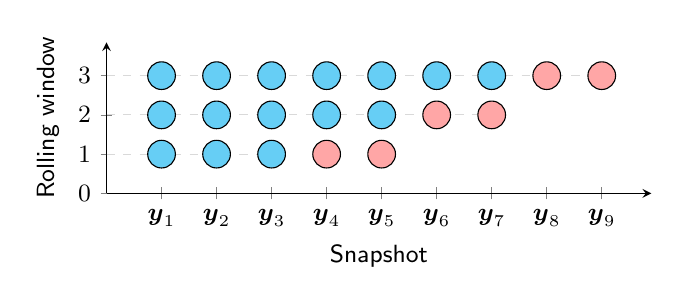
\begin{tikzpicture}[
    % Define reusable styles
    cyanmark/.style={only marks, mark size=5, color=cyan!60, draw=black},
    redmark/.style={only marks, mark size=5, color=red!35, draw=black},
    dashline/.style={dashed, color=gray!30, mark=none}
]
\begin{axis}[
    axis lines=left,
    enlargelimits=upper, 
    domain=0:2,
    xmin=0, ymin=0, ymax=3.5,
    xtick={1,...,9},
    xticklabels={
        $\boldsymbol{y}_{1}$, $\boldsymbol{y}_{2}$, $\boldsymbol{y}_{3}$,
        $\boldsymbol{y}_{4}$, $\boldsymbol{y}_{5}$, $\boldsymbol{y}_{6}$,
        $\boldsymbol{y}_{7}$, $\boldsymbol{y}_{8}$, $\boldsymbol{y}_{9}$
    },
    legend pos=outer north east,
    width=8.5cm,
    height=3.5cm,
    xlabel=Snapshot,
    ylabel=Rolling window,
    xlabel near ticks,
    ylabel near ticks,
    tick label style={font=\small},
    label style={font=\small}
]

% Add plots using defined styles
\addplot[cyanmark] coordinates{(1,1) (2,1) (3,1)};
\addplot[redmark]  coordinates{(4,1) (5,1)};
\addplot[cyanmark] coordinates{(1,2) (2,2) (3,2) (4,2) (5,2)};
\addplot[redmark]  coordinates{(6,2) (7,2)};
\addplot[cyanmark] coordinates{(1,3) (2,3) (3,3) (4,3) (5,3) (6,3) (7,3)};
\addplot[redmark]  coordinates{(8,3) (9,3)};

% Dashed lines
\addplot[dashline] coordinates{(0,1) (3,1)};
\addplot[dashline] coordinates{(0,2) (7,2)};
\addplot[dashline] coordinates{(0,3) (9,3)};

\end{axis}
\end{tikzpicture}
\end{document}
